\begin{frame}[plain]
  \begin{tikzpicture}[remember picture, overlay, shift={(current page.north west)}]

    \fill[argonneRed]
      (0.73mm, -0.77mm) rectangle ++(58.08mm, -5.81mm);
    \fill[argonneGreen]
      (2.18mm, -2.18mm) rectangle ++(72.59mm, -5.81mm);
    \fill[argonneBlue]
      (3.63mm, -3.63mm) rectangle ++(87.11mm, -5.81mm);
    \fill[white]
      (5.08mm, -5.08mm) rectangle ++(101.27mm, -7.30mm);

    \node[anchor=west,
          font=\fontsize{12}{14}\selectfont\bfseries,
          text width=96mm]
      at (7mm, -5.08mm - 7.30mm/2)
      {Baseline YAML Layout};

    \node[anchor=north west, inner sep=0pt]
      at (100mm, -3mm)
      {\includegraphics[width=25mm]{\argonneLogo}};

    \node[anchor=north west, inner sep=0pt]
      at (130mm, 1mm)
      {\includegraphics[width=25mm]{\atlasLogo}};

  \end{tikzpicture}

  \vspace{10mm}
  \begin{center}
    \begin{minipage}[t]{0.46\textwidth}
      \centering
      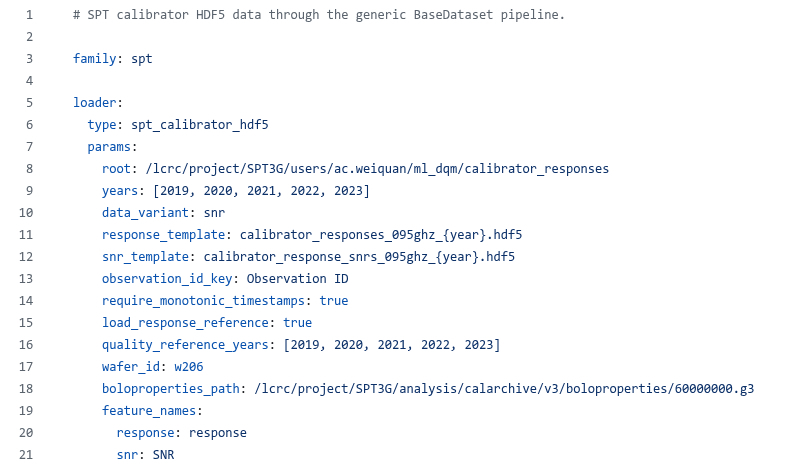
\includegraphics[width=\textwidth,height=52mm,keepaspectratio]{figures/loader.jpg}\\[0.5mm]
      {\fontsize{6.5}{7.5}\selectfont loader}\\[12.0mm]
      {\fontsize{7}{8.2}\selectfont
      \begin{minipage}{0.92\textwidth}
      {\setbeamertemplate{itemize item}{\color{black}-}
      \begin{itemize}
        \item Dynamic YAML layout is easy to review at a glance.
        \item Validated against existing pipeline.
      \end{itemize}}
      \end{minipage}}
    \end{minipage}
    \hfill
    \begin{minipage}[t]{0.46\textwidth}
      \centering
      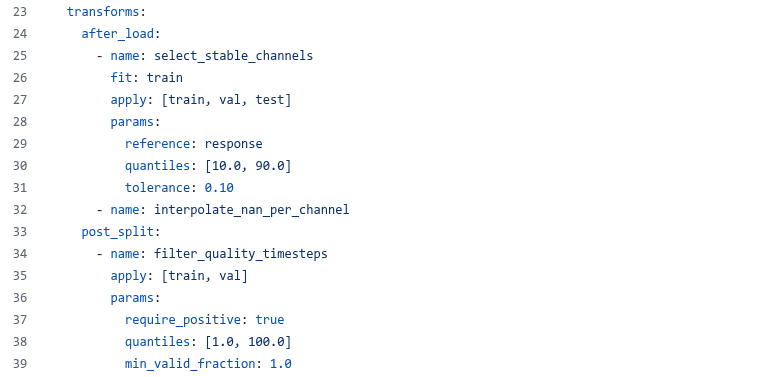
\includegraphics[width=\textwidth,height=31mm,keepaspectratio]{figures/transforms.jpg}\\[0.5mm]
      {\fontsize{6.5}{7.5}\selectfont transforms (after\_load, post\_split)}\\[1mm]
      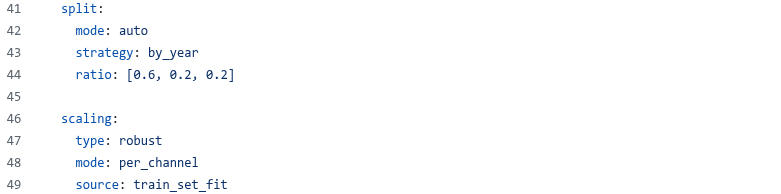
\includegraphics[width=\textwidth,height=15mm,keepaspectratio]{figures/post.jpg}\\[0.5mm]
      {\fontsize{6.5}{7.5}\selectfont split \& scaling}
    \end{minipage}
  \end{center}

  \vspace{1.5mm}
  \begin{center}
  {\fontsize{7}{8.3}\selectfont
  \href{https://github.com/anl-hep-ai-ml/CrossExperimentalAIDQM/blob/fd5c3da31b389d98656e1f63894bf32a99057724/src/anldq/configs/data_config/spt_configured.yml}{\texttt{spt\_configured.yml}}}
  \end{center}

  \slideheaderfooter
\end{frame}
